
%%%%%%%%%%%%%%%%%%%%%%%%%%%%%%%%%%%%%%%%%%%%%%%%%%%%%%%%%%%%%%%%%%%%%
%%                                                                 %%
%% Please do not use \input{...} to include other tex files.       %%
%% Submit your LaTeX manuscript as one .tex document.              %%
%%                                                                 %%
%% All additional figures and files should be attached             %%
%% separately and not embedded in the \TeX\ document itself.       %%
%%                                                                 %%
%%%%%%%%%%%%%%%%%%%%%%%%%%%%%%%%%%%%%%%%%%%%%%%%%%%%%%%%%%%%%%%%%%%%%

%%\documentclass[referee,sn-basic]{sn-jnl}% referee option is meant for double line spacing

%%=======================================================%%
%% to print line numbers in the margin use lineno option %%
%%=======================================================%%

%%\documentclass[lineno,sn-basic]{sn-jnl}% Basic Springer Nature Reference Style/Chemistry Reference Style

%%======================================================%%
%% to compile with pdflatex/xelatex use pdflatex option %%
%%======================================================%%

%%\documentclass[pdflatex,sn-basic]{sn-jnl}% Basic Springer Nature Reference Style/Chemistry Reference Style

%%\documentclass[sn-basic]{sn-jnl}% Basic Springer Nature Reference Style/Chemistry Reference Style
\pdfoutput=1
\documentclass[sn-mathphys]{sn-jnl}% Math and Physical Sciences Reference Style

%%\documentclass[sn-aps]{sn-jnl}% American Physical Society (APS) Reference Style
%%\documentclass[sn-vancouver]{sn-jnl}% Vancouver Reference Style
%%\documentclass[sn-apa]{sn-jnl}% APA Reference Style
%%\documentclass[sn-chicago]{sn-jnl}% Chicago-based Humanities Reference Style
%%\documentclass[sn-standardnature]{sn-jnl}% Standard Nature Portfolio Reference Style
%%\documentclass[default]{sn-jnl}% Default
%%\documentclass[default,iicol]{sn-jnl}% Default with double column layout

%%%% Standard Packages
%%<additional latex packages if required can be included here>
%%%%

%%%%%=============================================================================%%%%
%%%%  Remarks: This template is provided to aid authors with the preparation
%%%%  of original research articles intended for submission to journals published 
%%%%  by Springer Nature. The guidance has been prepared in partnership with 
%%%%  production teams to conform to Springer Nature technical requirements. 
%%%%  Editorial and presentation requirements differ among journal portfolios and 
%%%%  research disciplines. You may find sections in this template are irrelevant 
%%%%  to your work and are empowered to omit any such section if allowed by the 
%%%%  journal you intend to submit to. The submission guidelines and policies 
%%%%  of the journal take precedence. A detailed User Manual is available in the 
%%%%  template package for technical guidance.
%%%%%=============================================================================%%%%

\jyear{2023}%

%% as per the requirement new theorem styles can be included as shown below
\theoremstyle{thmstyleone}%
\newtheorem{theorem}{Theorem}%  meant for continuous numbers
%%\newtheorem{theorem}{Theorem}[section]% meant for sectionwise numbers
%% optional argument [theorem] produces theorem numbering sequence instead of independent numbers for Proposition
\newtheorem{proposition}[theorem]{Proposition}% 
%%\newtheorem{proposition}{Proposition}% to get separate numbers for theorem and proposition etc.

\theoremstyle{thmstyletwo}%
\newtheorem{example}{Example}%
\newtheorem{remark}{Remark}%

\newcommand{\appropto}{\mathrel{\vcenter{
  \offinterlineskip\halign{\hfil$##$\cr
    \propto\cr\noalign{\kern2pt}\sim\cr\noalign{\kern-2pt}}}}}

\theoremstyle{thmstylethree}%
\newtheorem{definition}{Definition}%
\usepackage{amsmath}
\usepackage{lineno}
\usepackage{subfig}
\usepackage{xcolor}
\usepackage{rotating}

\raggedbottom
%%\unnumbered% uncomment this for unnumbered level heads

\begin{document}
%\linenumbers
\renewcommand{\tablename}{Supplementary Table}
\renewcommand{\figurename}{Supplementary Figure}

\section{Supplemental materials}
\subsection{Tables and figures}
\begin{table}[h]
\begin{center}
\caption{Extension of Table 2 into a full ablation study encompassing the baseline supervised  model (PtychoNN, top row), PtychoPINN (bottom row), and two ablated versions of PtychoPINN, each containing one of the two defining features of the model (namely, ptychographic overlap constraints and the PINN/unsupervised structure).}\label{tab_ablation}
\begin{tabular}{p{2cm}l|ll|ll|ll}
\toprule
 & \multicolumn{1}{c}{} & \multicolumn{2}{c}{Lines} & \multicolumn{2}{c}{GRF} & \multicolumn{2}{c}{Large features}\\
\midrule
\bf{Feature set} & \bf{Metric}
& $\phi$ & $A$
& $\phi$ & $A$
& $\phi$ & $A$ \\
\midrule
$\{\}$\footnotemark[1]
& MAE & - & 0.201 & 0.0335 & 0.0153 & 0.219 & 0.0038 \\
& PSNR (dB) & - & 59.6 & 75.6 & 82.4 & 56.7 & 92.9 \\
& FRC50 ($\mathrm{pixel}^{-1}$) & - & 22.0 & 64.0 & 65.2 & 23.4 & 34.0 \\
\midrule
PINN
& MAE & - & 0.195 & 0.0859 & 0.0341 & 0.622 & 0.00581 \\
& PSNR (dB) & - & 59.7 & 67.5 & 75.4 & 50.3 & 88.8 \\
& FRC50 ($\mathrm{pixel}^{-1}$) & - & 22.0 & 29.7 & 64.7 & 8.2 & 13.9 \\
\midrule
overlaps
& MAE & - & 0.0755 & 0.0332 & 0.0158 & 0.187 & 0.00352 \\
& PSNR (dB) & - & 68.6 & 75.7 & 82.2 & 58.5 & 93.8 \\
& FRC50 ($\mathrm{pixel}^{-1}$) & - & 65.8 & 63.5 & 65.0 & 27.6 & 35.9 \\
\midrule
PINN,overlaps\footnotemark[2]
& MAE & - & \textbf{0.0473} & \textbf{0.0109} & \textbf{0.00507} & \textbf{0.149} & \textbf{0.00303} \\
& PSNR (dB) & - & \textbf{72.6} & \textbf{85.2} & \textbf{91.9} & \textbf{60.6} & \textbf{95.0} \\
& FRC50 ($\mathrm{pixel}^{-1}$) & - & \textbf{165.4} & \textbf{171.5} & \textbf{171.3} & \textbf{93.7} & \textbf{38.7} \\
\midrule
\end{tabular}
\end{center}
\footnotetext[1]{supervised baseline}
\footnotetext[2]{full PtychoPINN}
\end{table}


\begin{figure}
    \centering
    \subfloat{{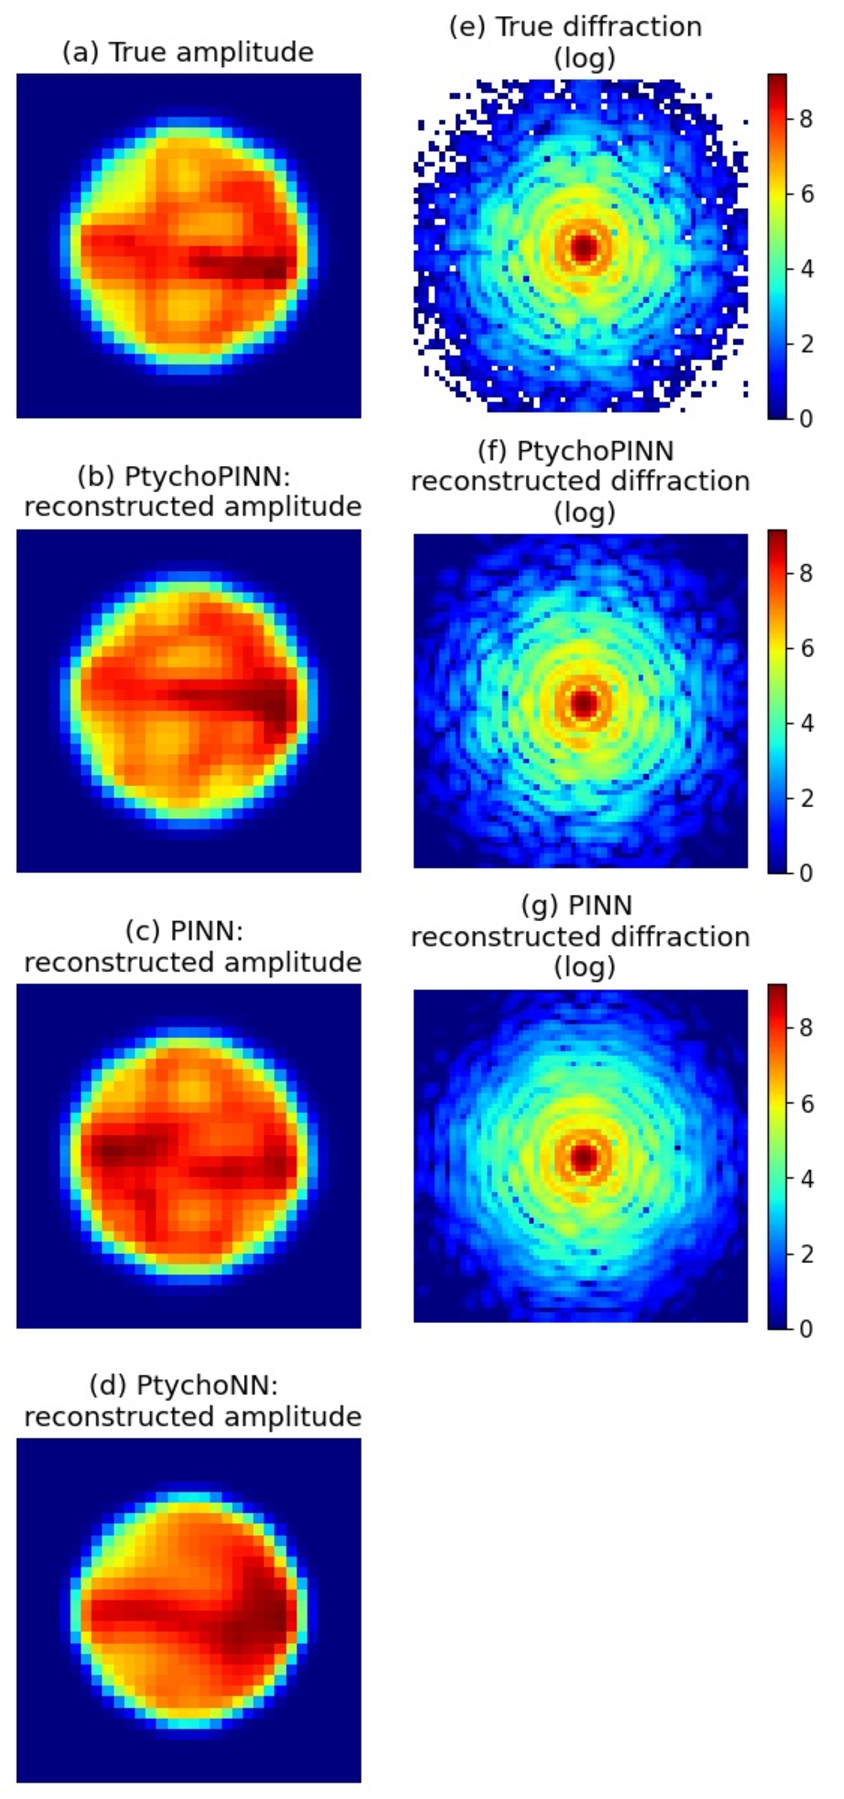
\includegraphics[width=6.5cm]{patches.pdf} }}
    \caption{\emph{PINN and parity}. Comparison of real-space and diffraction reconstructions from PtychoPINN (b) and the basic PINN (c) with no overlap constraints. Note that both PtychoPINN and the basic PINN reconstruct small features, but only PtychoPINN resolved the inversion degeneracy correctly. The supervised-training baseline (d) produces a reconstruction that has the correct asymmetry, but is considerably blurred.}%
    \label{fig:patches}
\end{figure}

\subsection{Plotting details}
All amplitudes images are plotted with an auto-scaled color map. Because the model introduces a training run-specific normalization factor into reconstructed amplitudes, we omit numerical scales in the presentation of amplitude images.



\end{document}
